\documentclass[12pt]{article}

\usepackage{sbc-template}

\usepackage{graphicx,url}

\usepackage[brazil]{babel}   	
%\usepackage[latin1]{inputenc}  
\usepackage[utf8]{inputenc}

\graphicspath{{./img/}}
% UTF-8 encoding is recommended by ShareLaTex 			

% \usepackage{natbib}
% 
% \setcitestyle{authoryear, open={((},close={))}}
     
\sloppy

\title{Sistemas Gerenciadores de Conteúdo e de Aprendizagem}

\author{Inalberth P. Santos\inst{1}, Ramon C. Gusmão\inst{1}, Ramon V. S. Bezerra\inst{1}}

\address{Instituto Federal de Educação, Ciência e Tecnologia do Maranhão\\
  Av. Getúlio Vargas, 04 -- São Luís -- MA -- Brasil
  \email{\{inalberth07, ramoncgusmao, ramonbezerra90\}@gmail.com}
}

\begin{document} 
    
\maketitle

\begin{abstract}
  The purpose of this paper is present Content and Learning Management Systems, which are organised in three basic categories: content, learning and the third one 
  based on content and learning, explaining their origins, characteristics, usage and relations among them, as well as showing their similarities 
  and differences, since even today such terms are used incorrectly, contributing to a possible wrong choice for a company or educational 
  institution to acquire such a project.
\end{abstract}
     
\begin{resumo} 
  O objetivo deste artigo é apresentar os Sistemas de Gerenciamento de Conteúdo e Aprendizagem, os quais se dividem em três categorias básicas:
  conteúdo, aprendizado e o terceiro baseado em ambos aprendizado e conteúdo, abordando suas origens, características, aplicações e por fim 
  relacioná-los, exibindo suas semelhanças e diferenças, visto que mesmo hoje o emprego destes termos ocorre de maneira incorreta, o que pode 
  resultar em uma escolha equivocada para uma empresa ou instituição de ensino ao conceber um projeto deste segmento.
\end{resumo}

\section{Introdução} \label{sec:introducao}

Segundo \cite{phillipo2012link}, os sistemas gerenciadores de conteúdo e aprendizagem são o \emph{``elo perdido''} que interliga as reformas na 
educação contemporânea com o uso criativo e efetivo da tecnologia, porém, esta por si só não é capaz de promover aprendizado. 
Logo os sistemas os quais são objeto de estudo deste trabalho se apresentam como ferramentas que possibilitam ao instrutor orientar e 
gerenciar os objetivos alcançados pelos estudantes de maneira mais eficiente. Neste trabalho serão apresentados os principais sistemas de 
gerenciamento de conteúdo e aprendizado: \emph{LMS} (gerenciador de aprendizado), \emph{CMS} (gerenciador de cursos) e \emph{LCMS} (gerenciador de conteúdos de 
aprendizagem), descrevendo suas origens, características e arquitetura, aplicações e a relação entre os mesmos, ressaltando-se o fato de que, 
apesar de haver consenso na definição de cada um, é comum o emprego incorreto dos termos.

\section{LMS (\textit{Learning Management Systems})} \label{sec:lms}

Os LMS (do inglês, \textit{Learning Management Systems}) são aplicações de \textit{software} baseadas em tecnologias Web ou não, utilizadas para 
planejar, implementar e dar suporte ao processo de aprendizagem. A TalentLMS -- plataforma de aprendizado virtual utilizada por diversas 
organizações em segmentos distintos -- faz em sua página uma breve explanação das 
palavras que compõem o termo\footnote{http://www.talentlms.com/what-is-an-lms/\#what-is-an-lms}:

\begin{itemize}
 \item \textbf{Learning,} porque você utiliza-os para entregar/receber programas de treinamento e/ou cursos educacionais, 
 \item \textbf{Management,} porque ajuda você a organizar estes cursos, isto é, criar, alterar,
 \item \textbf{System, } porque é um programa de computador.
\end{itemize}

Conforme \cite{lonn2009saving}, LMS são sistemas Web que permitem aos instrutores/alunos compartilhar materiais, enviar e receber tarefas, fazer 
apontamentos de aulas e se comunicar online. 

Desta maneira, observa-se consenso na literatura quanto à definição do termo, porém, apesar de 
conhecida a expressão, a mesma é empregada incorretamente com certa frequência, assim como confundida com outros dois tipos de gerenciadores: 
CMS e LCMS, os quais serão abordados nas seções seguintes.

\subsection{Origens}

Segundo \cite{watson2007learning}, a sigla LMS tem sua origem na expressão ILS (\textit{Integrated Learning System}), termo criado pela Jostens 
Learning, o qual faz referência a funcionalidades adicionais além dos recursos instrucionais, como gerenciamento de conteúdo e monitoramento. 
Já LMS foi utilizado pela primeira vez para descrever parte do sistema de gerenciamento do sistema de aprendizagem PLATO K-12.

\subsection{Características}

Em termos educacionais, constitui um LMS, conforme visto em \cite{bailey1992wanted}:

\begin{itemize}
 \item Objetos de Aprendizagem são organizados em lições individuais
 \item Aulas são agrupadas em um plano de ensino
 \item Um sistema de gerenciamento coleta os resultados do desempenho do estudante
 \item Aulas são disponbilizados aos alunos de acordo com o seu progresso na aprendizagem
\end{itemize}

Assim como outros \textit{softwares}, estes sistemas podem ser aplicados em um ambiente corporativo. A seguir são listadas as características 
recomendadas para a composição do mesmo, segundo a Sociedade Americana de Treinamento e Desenvolvimento:

\begin{itemize}
 \item Integração com o Sistema de Recursos Humanos.
 \item Ferramentas de administração que possibilitem o gerenciamento dos registros de usuários, perfis, conteúdos, orçamentos, agendamento para 
 aprendizes, tutores e salas de aula.
 \item Disponibilização de acesso ao conteúdo envolvendo o meio (sala de aula, \textit{online}), método (através de um orientador, 
 somente aprendiz) e aprendizes (alunos, clientes).
 \item Desenvolvimento de conteúdo (autoria, manutenção e armazenamento)
 \item Integração de conteúdo com \textit{software} de aprendizagem de terceiros
 \item Adoção dos modelos SCORM e AICC, os quais permitem importar gerenciar conteúdos seguindo padrões independentemente dos sistemas de 
 autoria utilizados para criá-los.
\end{itemize}

Conforme \cite{watson2007learning}, o ponto principal para entender as diferenças entre LMS e outros termos relacionados à educação utilizando 
computador é compreender a natureza sistêmica dos LMS, reforçando a ideia de que este é um \textit{framework} responsável por gerenciar todos 
os aspectos do processo de aprendizagem, não se limitando, portanto, apenas à disponibilização de conteúdo, mas fazendo o gerenciamento dos 
usuários, salas de aula, cursos, análise de desempenho dos estudantes/aprendizes, acompanhando o progresso obtido, coletando e apresentando os 
dados para supervisionar o processo de aprendizagem da organização como um todo.

\subsubsection{Vantagens}

São listadas a seguir algumas das vantagens desta categoria de sistemas, apresentadas pela Mindflash\footnote{https://www.mindflash.com/lms}, 
empresa que promove treinamentos para diversas empresas:

\begin{itemize}
 \item Fácil adaptação e reuso de materiais.
 \item Mais opções para os criadores dos cursos como métodos de disponibilização, design de materiais, técnicas de avaliação.
 \item Redução de custos relacionados aos gastos com o desenvolvimento e manutenção de conteúdo por terceiros.
 \item Melhoria no desenvolvimento profissional e avaliação, permitindo a maior agregação de valor aos Recursos Humanos das companhias e ao mesmo 
 proporcionando aos empregados seu desenvolvimento individual.
\end{itemize}

\section{CMS (\textit{Content Management Systems})}

\section{LCMS (\textit{Learning Content Management Systems})}

\section{Relação entre LMS, CMS e LCMS}

Como já mencionado, por muitas vezes os termos estudados são utilizados incorretamente. Conforme visto em \cite{watson2007learning}, o uso 
inadequado do termo LMS na literatura é frequentemente associado a aplicações identificadas como CMS. O mesmo autor relata que esta modalidade é 
utilizada principalmente para aprendizado online, possuindo suporte para inclusão de material online, associar alunos com cursos, monitorar o 
desempenho dos estudantes/aprendizes, armazenar as submissões, funcionalidades as quais podem ser encontradas em um LMS, permitindo a confusão em 
definir/diferenciar os dois tipos de sistema.

\bibliographystyle{sbc}
\bibliography{referencias}

\newpage
\appendix
\section{Linha do Tempo dos LMS}

% \begin{figure}[ht]
% \centering
% 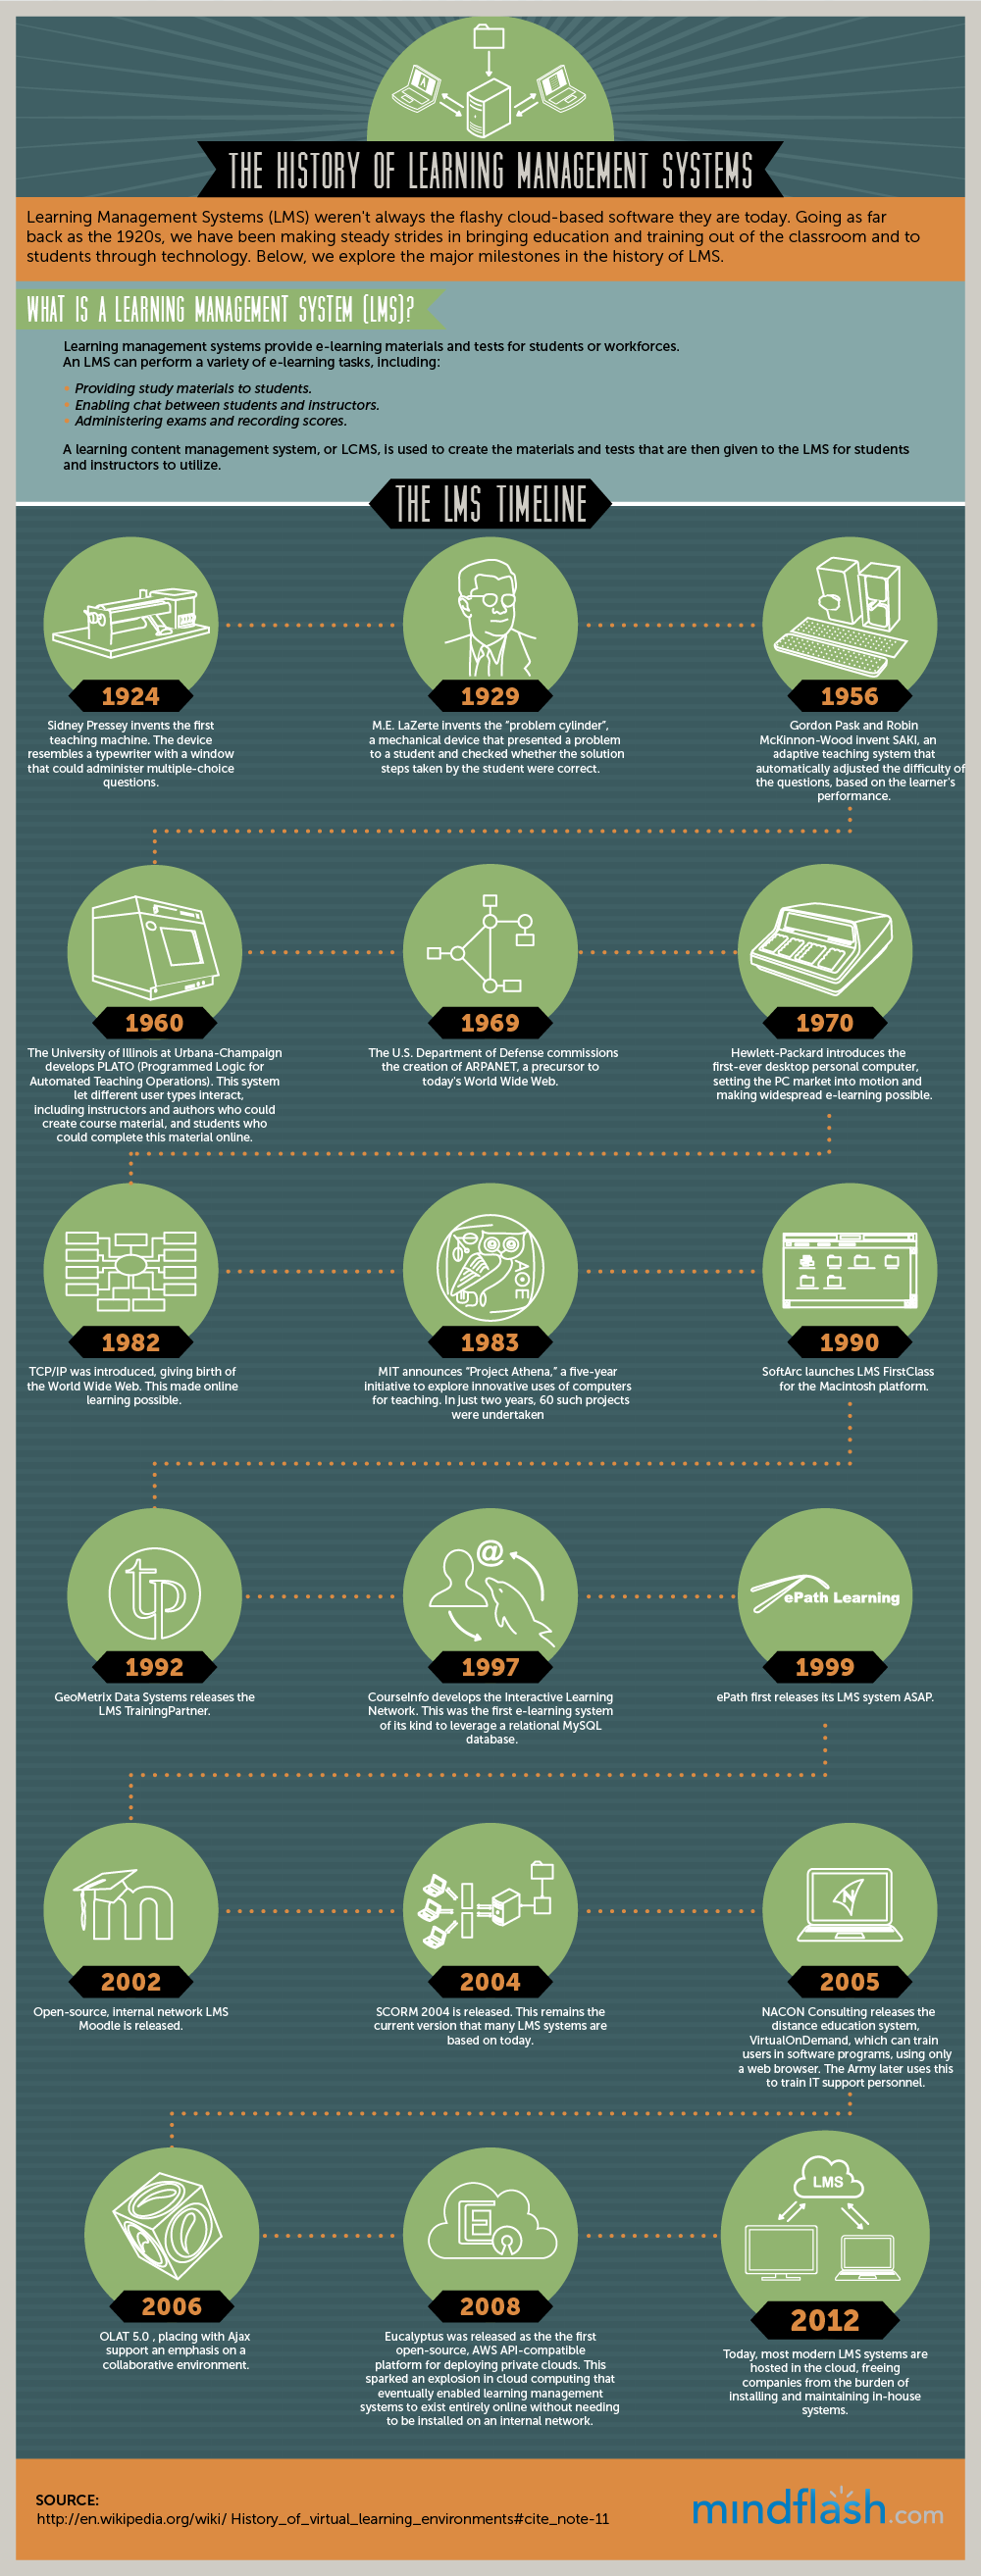
\includegraphics[width=.55\textwidth]{history-of-lms.png}
% \caption{A typical figure}
% \label{fig:exampleFig1}
% \end{figure}

\end{document}
